\documentclass[12pt]{article}
\usepackage[margin=2cm]{geometry}

\usepackage{graphicx}
\usepackage{array}
\usepackage{url}
\usepackage{multicol}
\usepackage{amsmath}
\usepackage{amssymb, amsfonts, amsthm}

\begin{document}

\begin{figure}
    \centering
    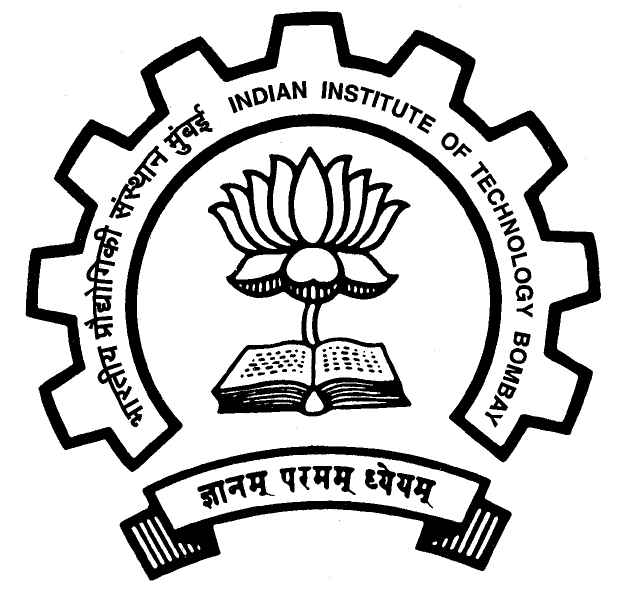
\includegraphics[width=5cm]{iitb-logo.png}
\end{figure}

\begin{center}
    \textbf{\LARGE Indian Institute of Technology Bombay} \\
    \vspace{1cm}
    \Large Project Report\\
    \vspace{0.3cm}

    \rule{\linewidth}{0.5pt} \\
    \vspace{0.2cm}
    \textbf{\LARGE AE 308 \\ \vspace{0.3cm} Control Theory} \\
    \vspace{0.1cm}
    \rule{\linewidth}{0.5pt} \\
    \vspace{1.5cm}
    \LARGE Compensator Design\\

    \vspace{2cm}

    \normalsize Ravi Kumar \\
    210010052

    \vspace{3cm}

    \normalsize\textit{Course Instructor:}\vspace{0.2cm}
    Prof. Arnab Maity

    \vspace{1cm}
    \date{}
\end{center}

\newpage

\section{Introduction}
The given system is a third order type one system with a zero at origin and two
poles at $-10$ and $-1$. The transfer function of the system is given by:
$$G(s) = \dfrac{K}{s(0.1s+1)(s+1)}$$

Bode plot and root locus of the system (taking $K=4$):
\begin{figure}[h!]
    \centering
    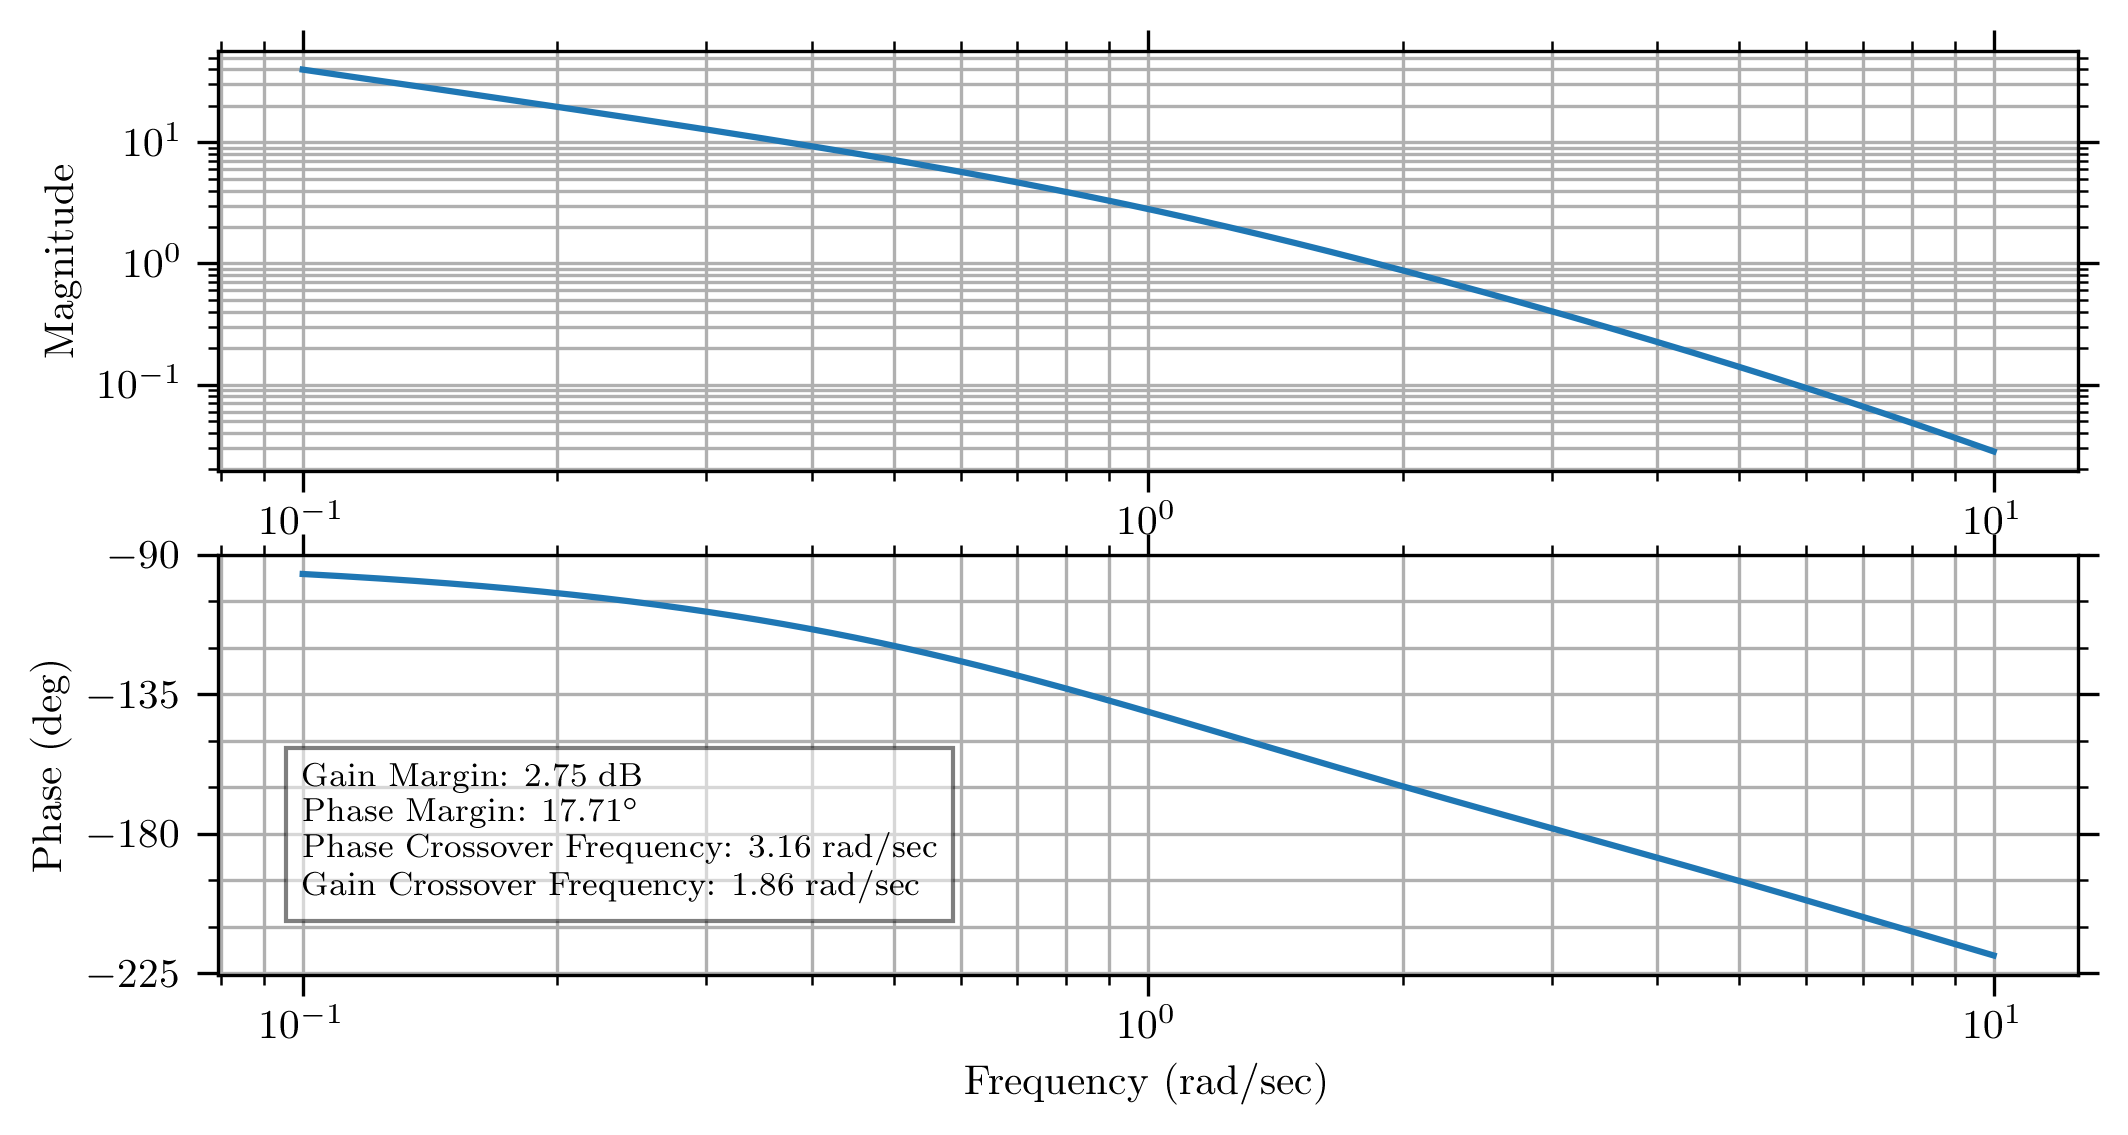
\includegraphics[width=0.8\linewidth]{bode_uncompensated.png}
    \caption {Bode plot of the uncompensated system}
    \label{fig:bode_uncompensated}
\end{figure}

\begin{figure}[h!]
    \centering
    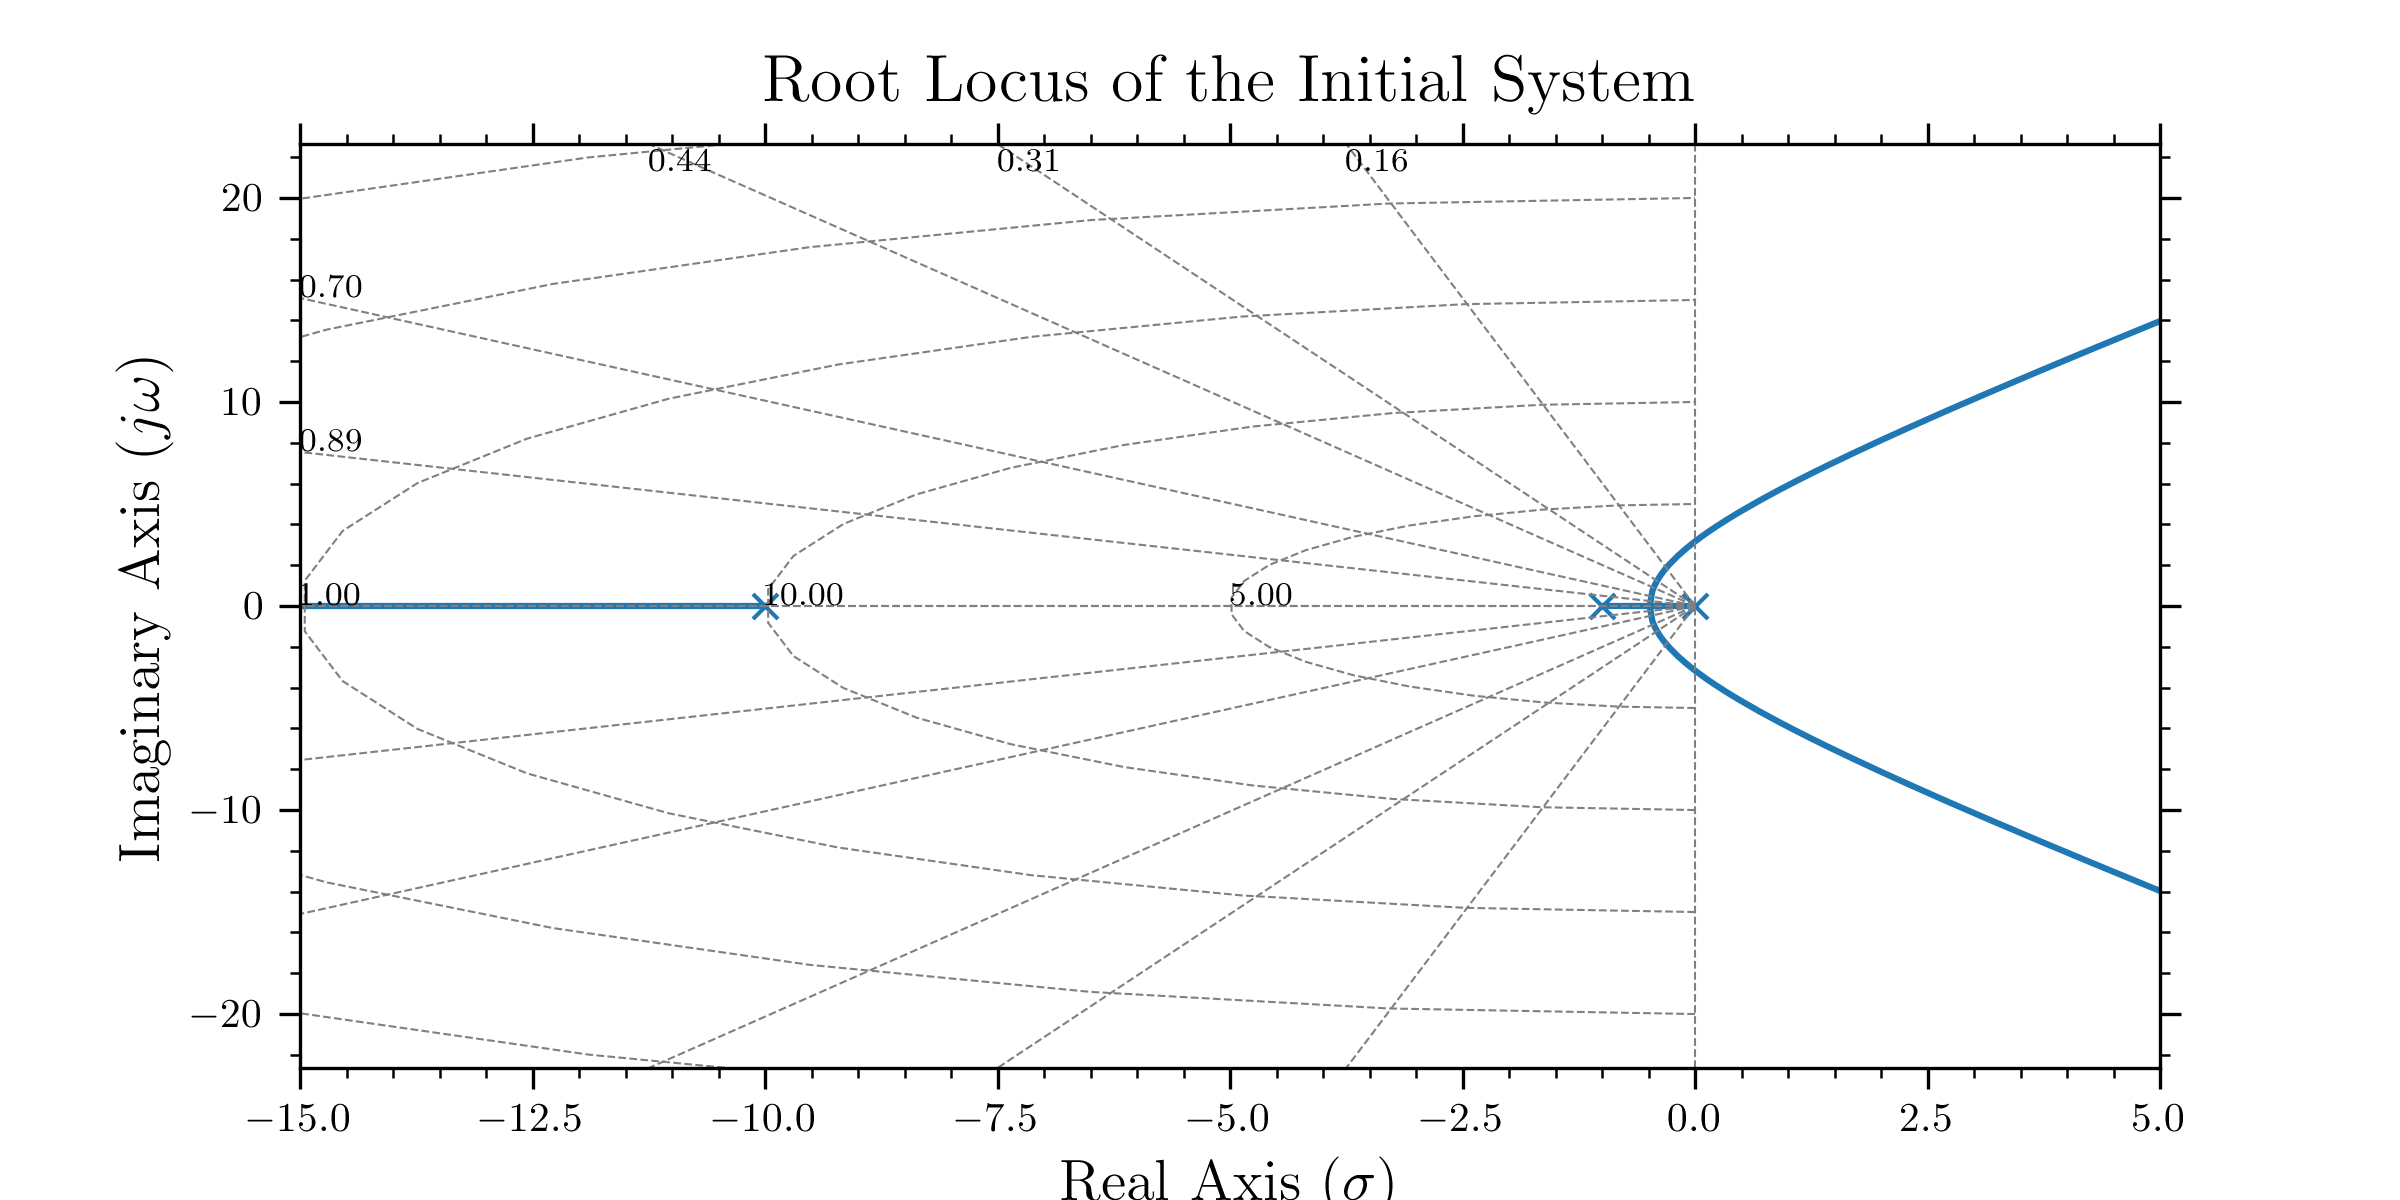
\includegraphics[width=0.8\linewidth]{rootlocus_uncompensated.png}
    \caption {Root locus of the uncompensated system}
    \label{fig:root_locus_uncompensated}
\end{figure}

\clearpage

Step response of the system (taking $K=4$):
\begin{figure}[h!]
    \centering
    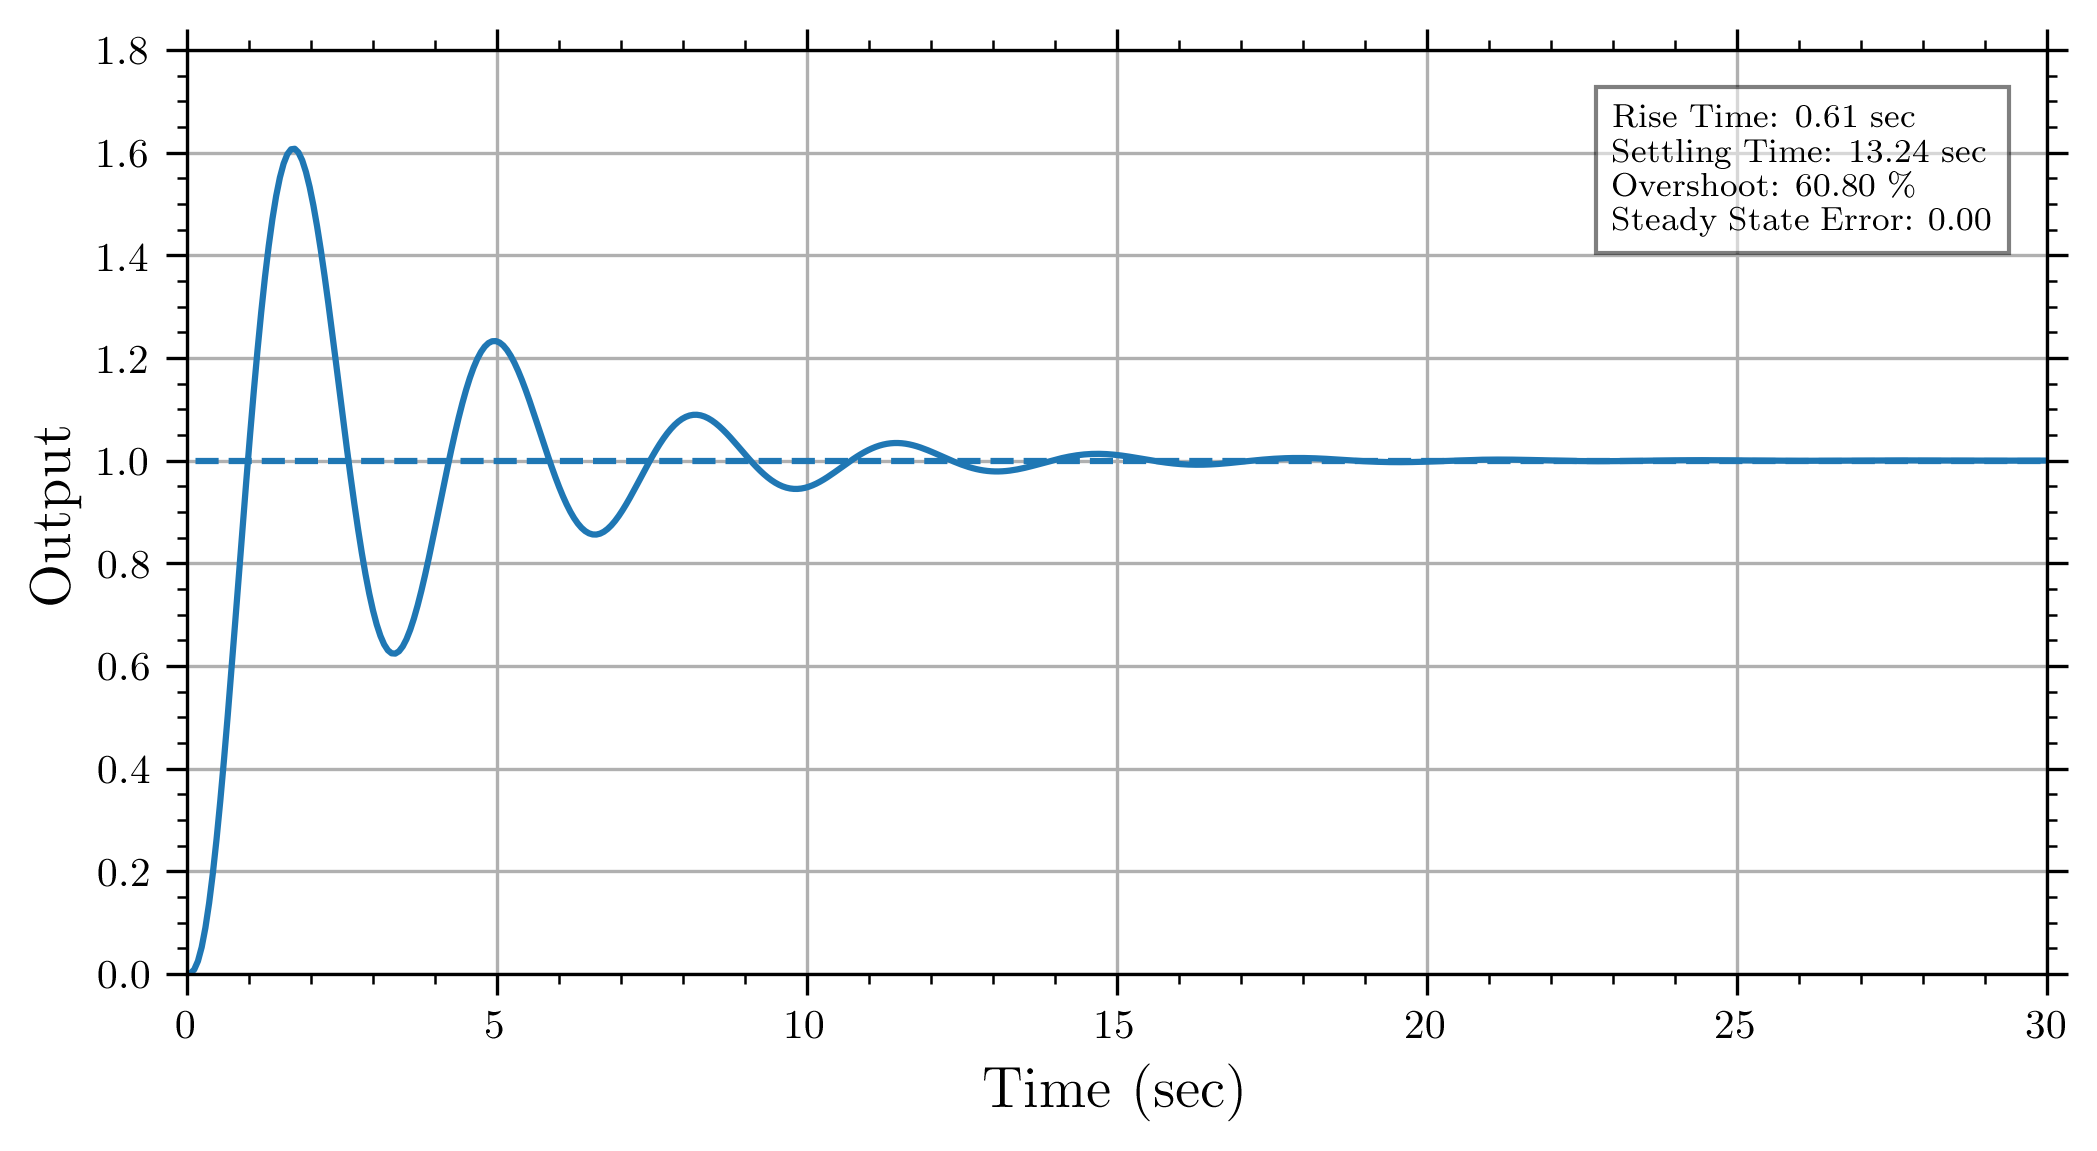
\includegraphics[width=0.8\linewidth]{step_response_uncompensated.png}
    \caption {Step response of the uncompensated system}
    \label{fig:step_uncompensated}
\end{figure}

Ramp response of the system (taking $K=4$):
\begin{figure}[h!]
    \centering
    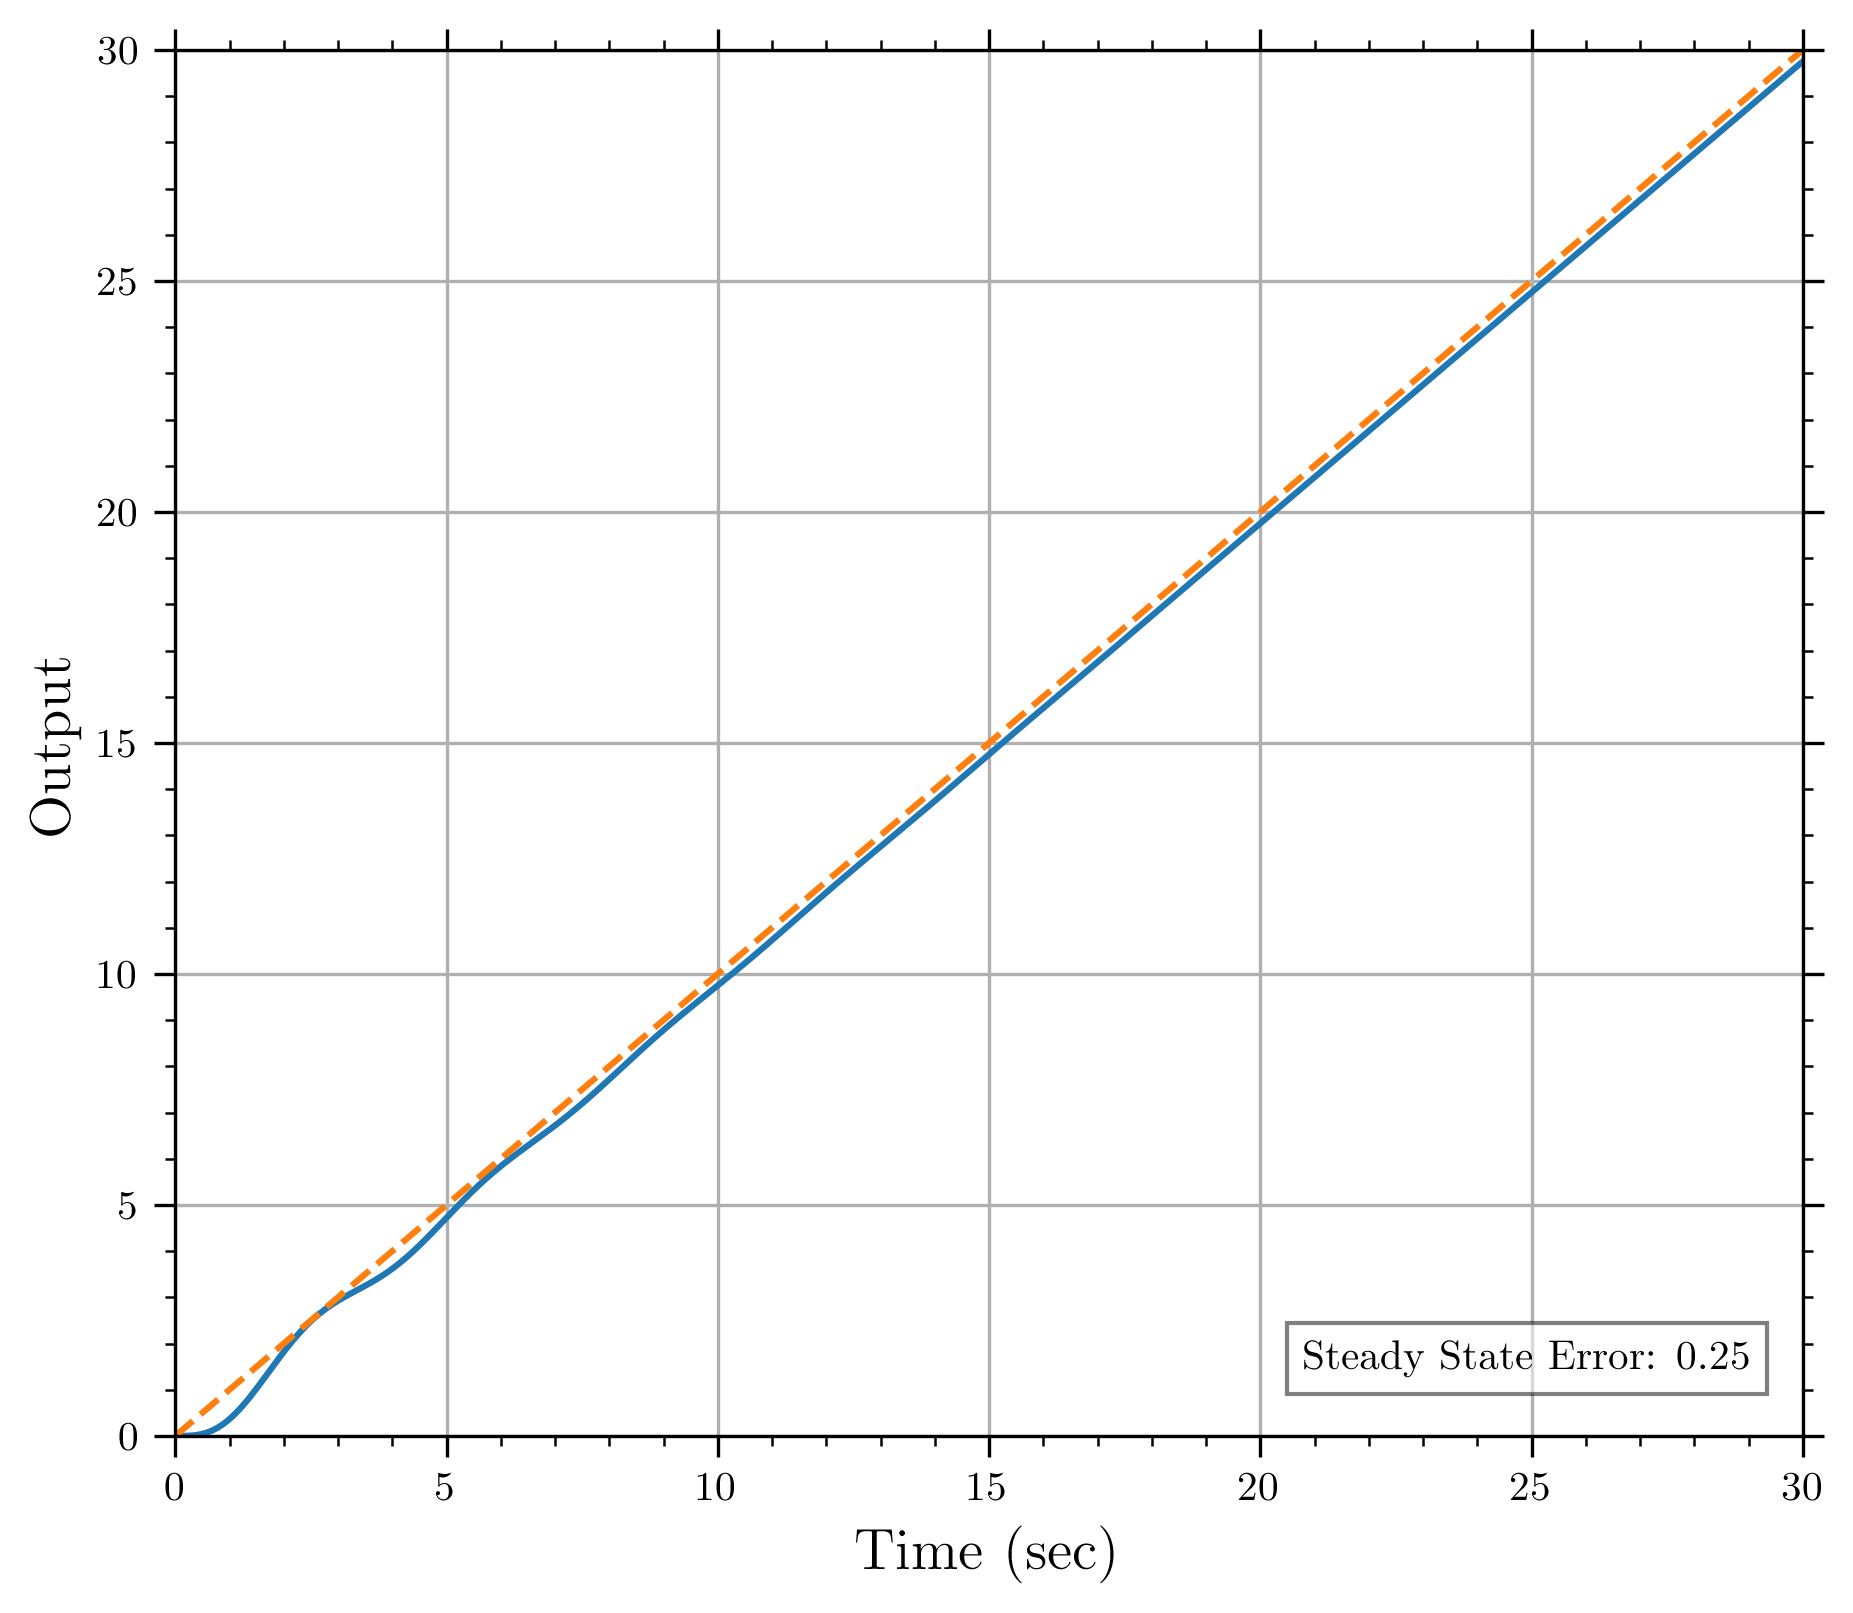
\includegraphics[width=0.7\linewidth]{ramp_response_uncompensated.png}
    \caption {Ramp response of the uncompensated system}
    \label{fig:ramp_uncompensated}
\end{figure}

\clearpage
\section{Control Objectives}
The following control objectives are to be achieved:
\begin{enumerate}
    \item Static velocity error constant ($K_v$) should be $4.0$ sec$^{-1}$
    \item Phase margin should be greater than $45^{\circ}$
    \item Gain margin should be greater than or equal to $8$ dB
\end{enumerate}

\section{Compensator Design}
According to the objectives, we will determine the value of K to yield the
desired static velocity error constant.

$$K_v = \lim_{s\to 0} sG(s) = K = 4$$

$\therefore$ Our uncompensated system is $G(s) = \dfrac{4}{s(0.1s+1)(s+1)}$

\subsection*{Bode Plot Method}
The system's initial phase margin is $17.71^\circ$. The required phase margin
should be greater than $45^\circ$. So, we need an additional phase of
$27.29^\circ$.

For safety, we will take the phase margin to be $50^\circ$. The $\omega$ for
which the phase margin is $50^\circ$ is $0.723$ rad/sec. At this frequency, we
get a gain of $13.01$ dB.

$$\implies w_{50} = 0.723 \text{rad/sec}$$
$$|G(jw_{50})| = 13.01 \text{dB}$$

\noindent Now, as a general rule, we add the zero a decade before the desired $w$, i.e.
at $w=\frac{w_{50}}{10}$ in a lag compensator. So, location of the zero is $-0.0723$. We also want gain at this frequency to be lowered by $13.01$ dB. Using this information, the location of pole is as follows:

$$20\log_{10}\left[{\dfrac{\text{zero}}{\text{pole}}}\right] = |G(jw_{50})|$$
$$\text{pole} = \text{zero}\times10^{\tfrac{-|G(jw_{50})|}{20}}$$

$$\therefore \text{pole}= -0.0723\times10^{\tfrac{-13.01}{20}} = -0.0162 $$

\noindent The transfer function of the lag compensator is given by:
$$G_c(s) = K_c\left[\dfrac{s+0.0723}{s+0.0162}\right]$$

Using $K_c$ as $\dfrac{\text{pole}}{\text{zero}}$ to get unity gain for
compensator, we finally get the following transfer function:

$$G_c(s) = 0.224\left[\dfrac{s+0.0723}{s+0.0162}\right]$$

Overall transfer function of the compensated system is given by: $$G_c(s) \cdot
    G(s) =
    \dfrac{4\times0.224}{s(0.1s+1)(s+1)}\left[\dfrac{s+0.0723}{s+0.0162}\right]$$

\section{Simulation Results}
Bode plot and root locus of the compensated system:
\begin{figure}[h!]
    \centering
    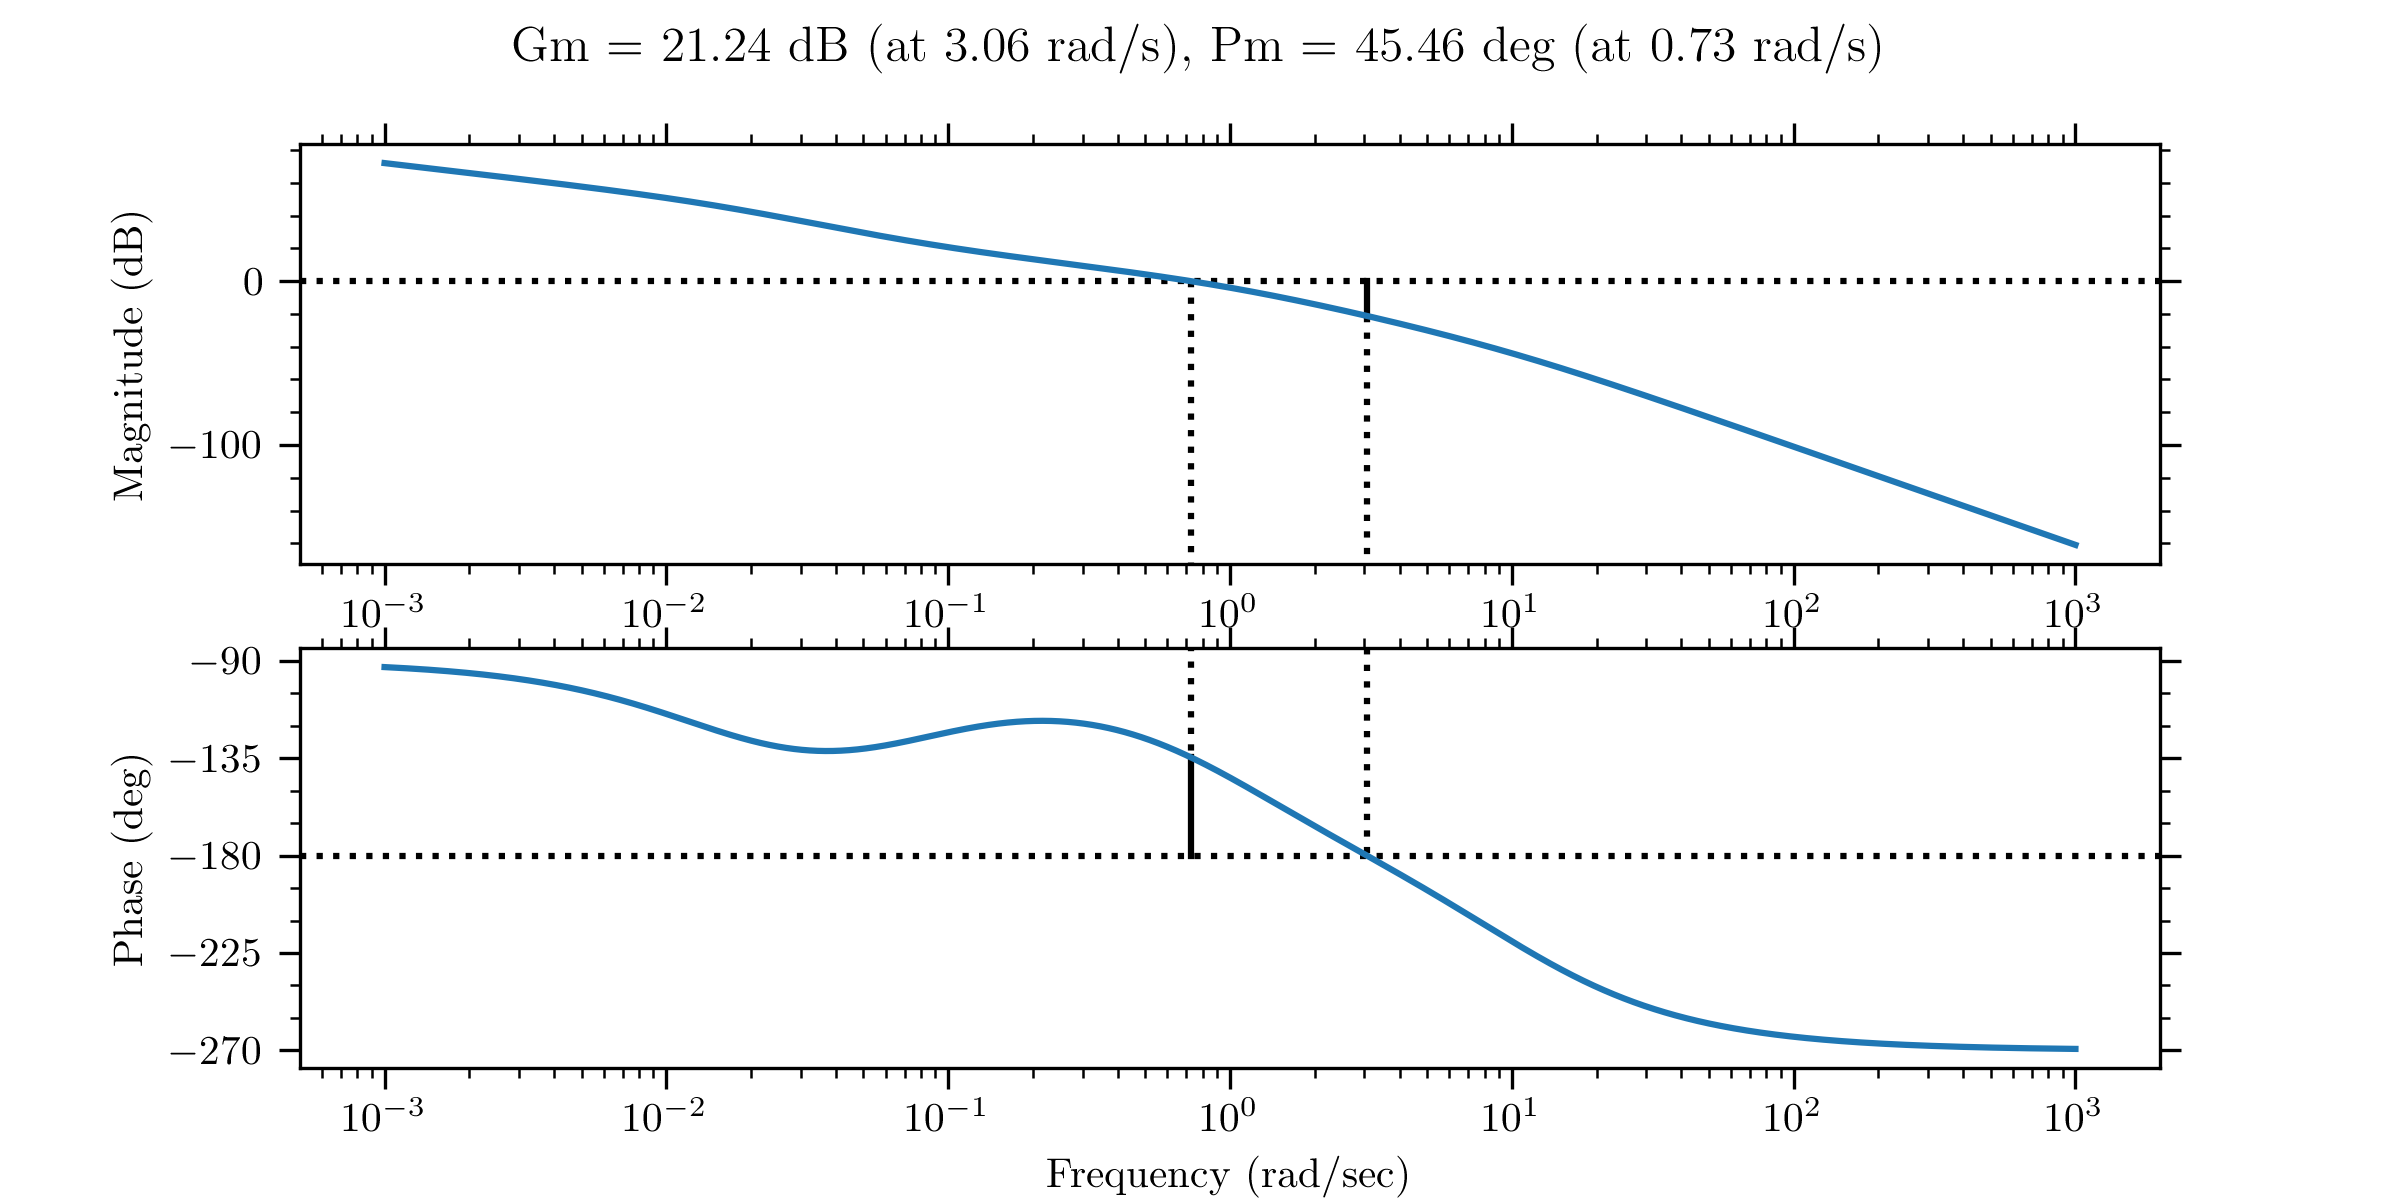
\includegraphics[width=0.8\linewidth]{bode_compensated.png}
    \caption {Bode plot of the compensated system}
    \label{fig:bode_compensated}
\end{figure}

\begin{figure}[h!]
    \centering
    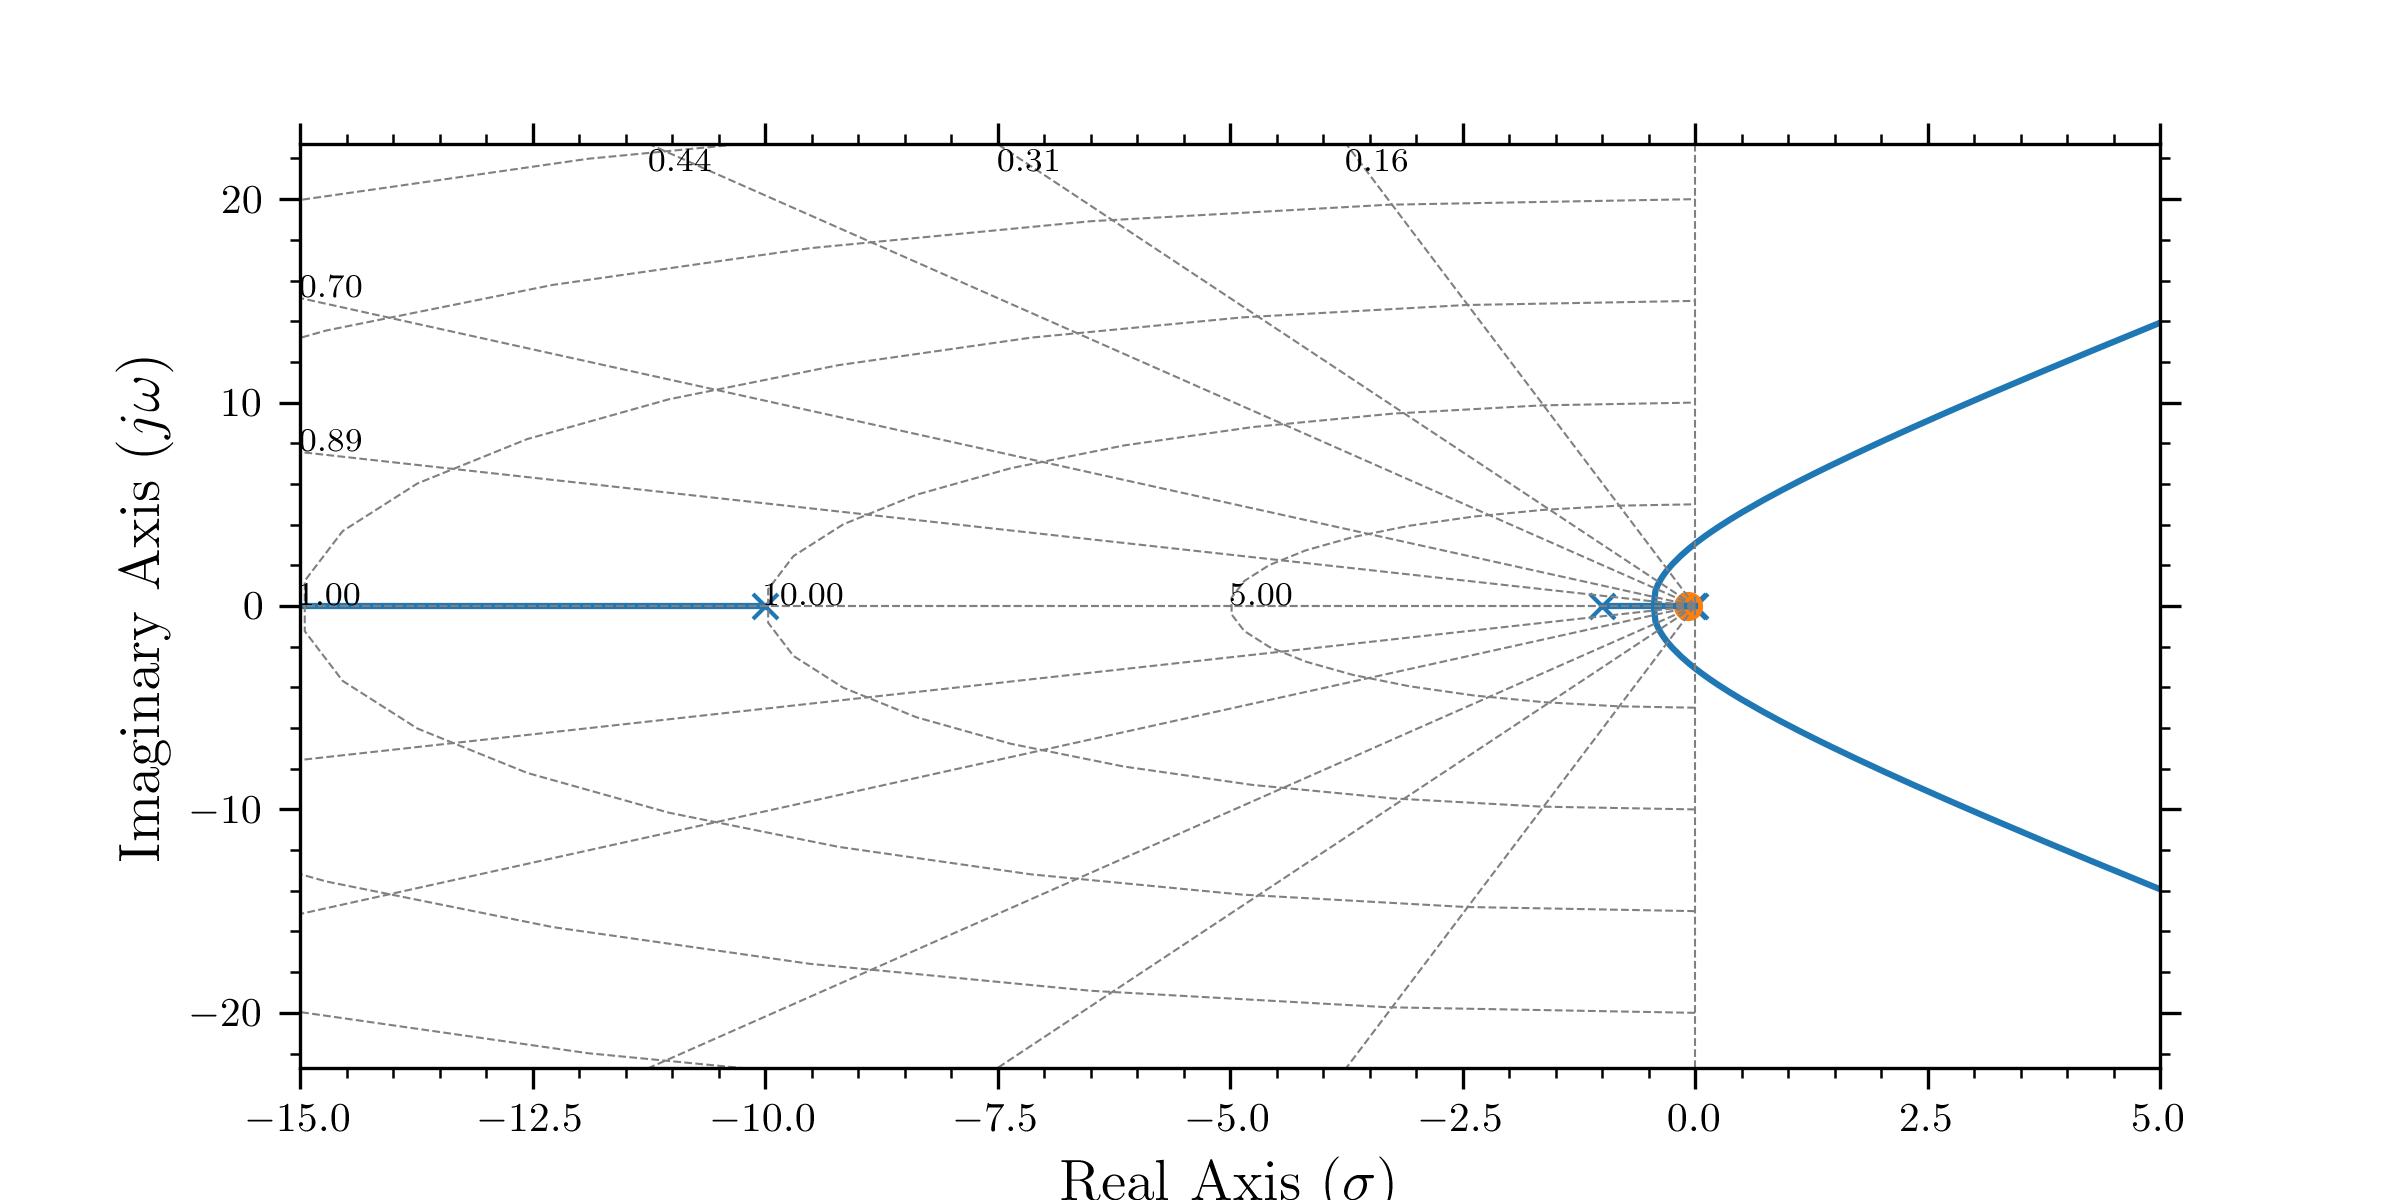
\includegraphics[width=0.8\linewidth]{rootlocus_compensated.png}
    \caption {Root locus of the compensated system}
    \label{fig:root_locus_compensated}
\end{figure}

\clearpage

Step response of the compensated system:
\begin{figure}[h!]
    \centering
    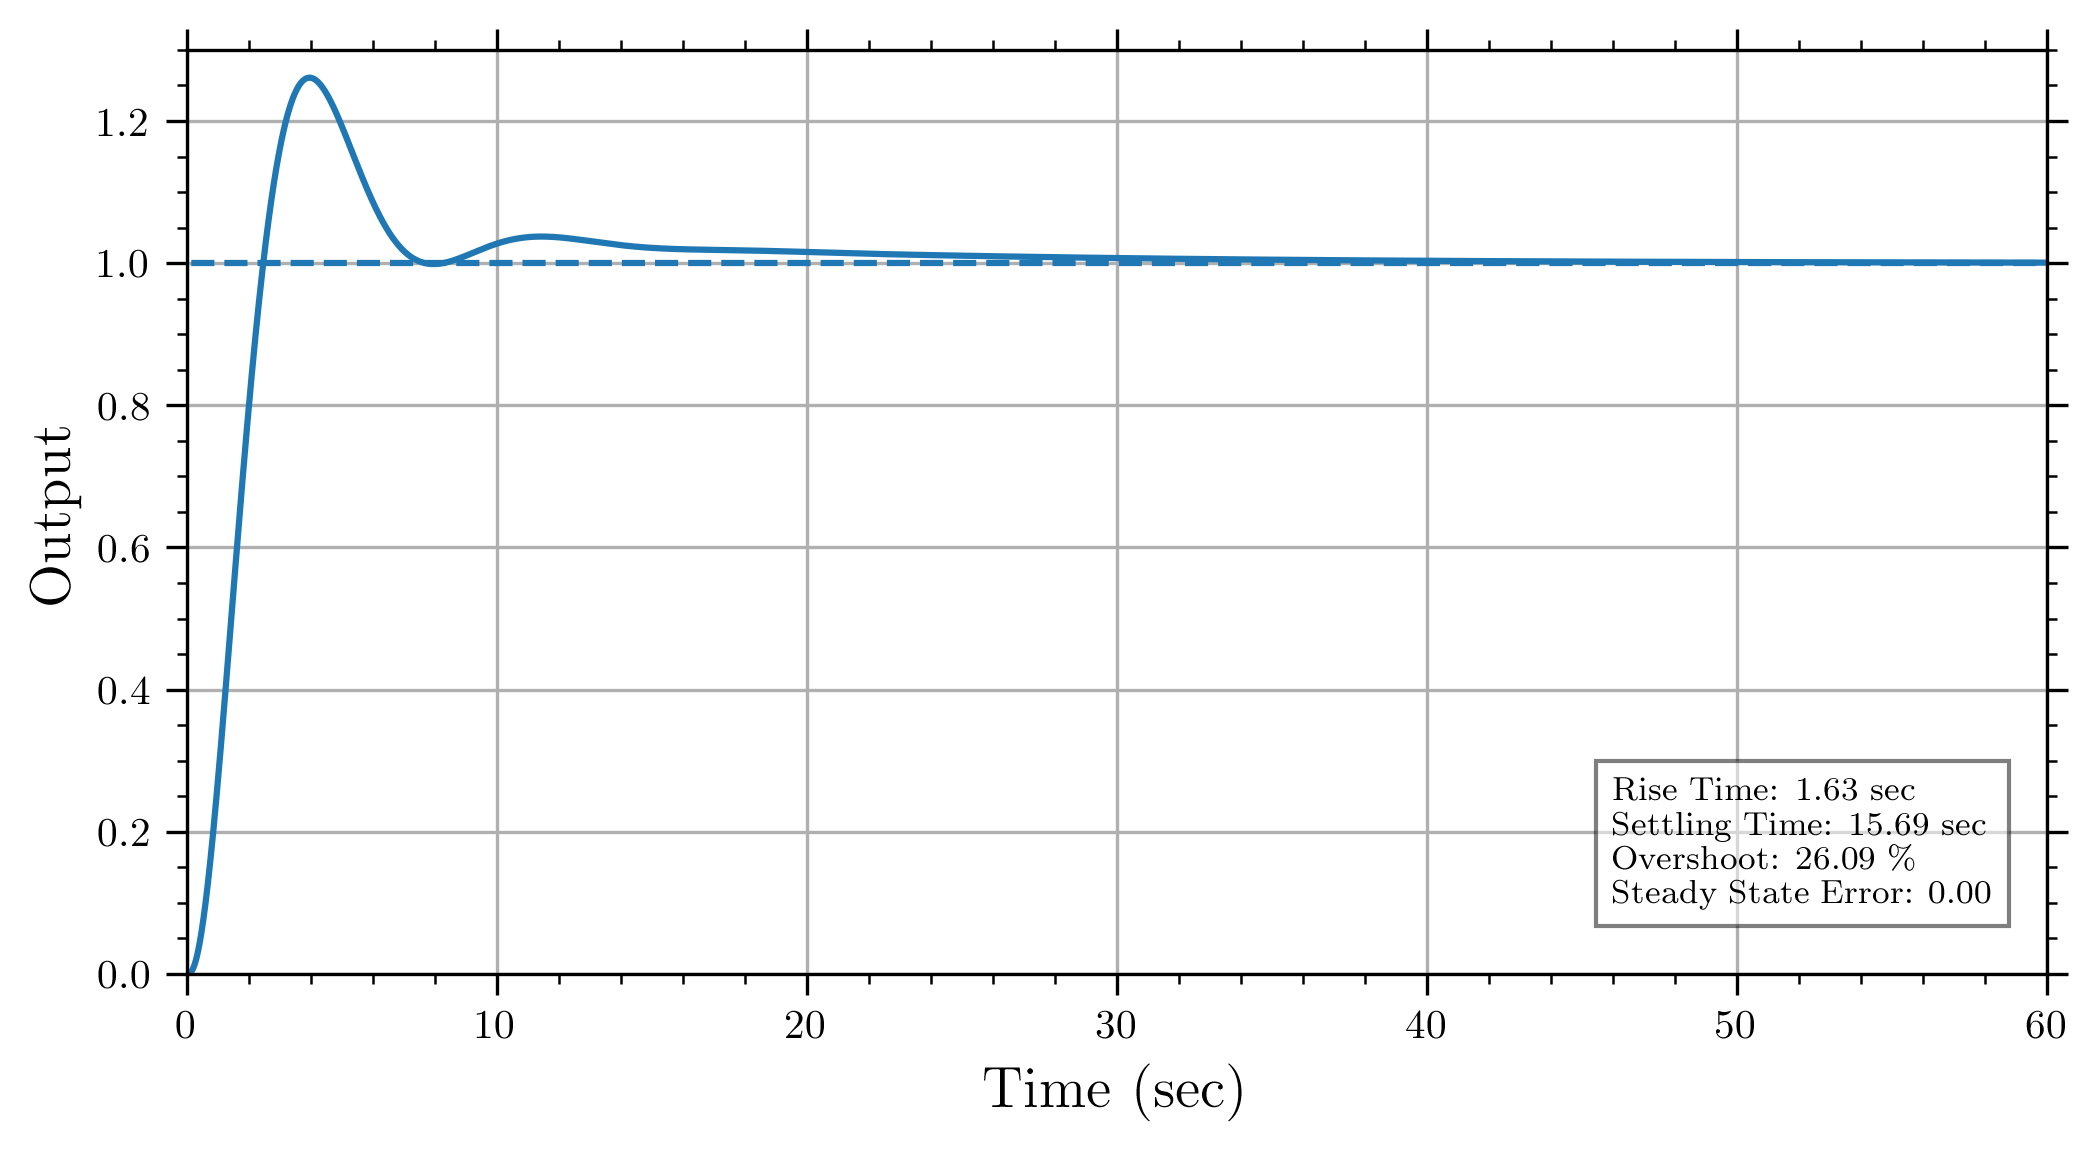
\includegraphics[width=0.8\linewidth]{step_response_compensated.png}
    \caption {Step response of the compensated system}
    \label{fig:step_compensated}
\end{figure}

Ramp response of the compensated system:
\begin{figure}[h!]
    \centering
    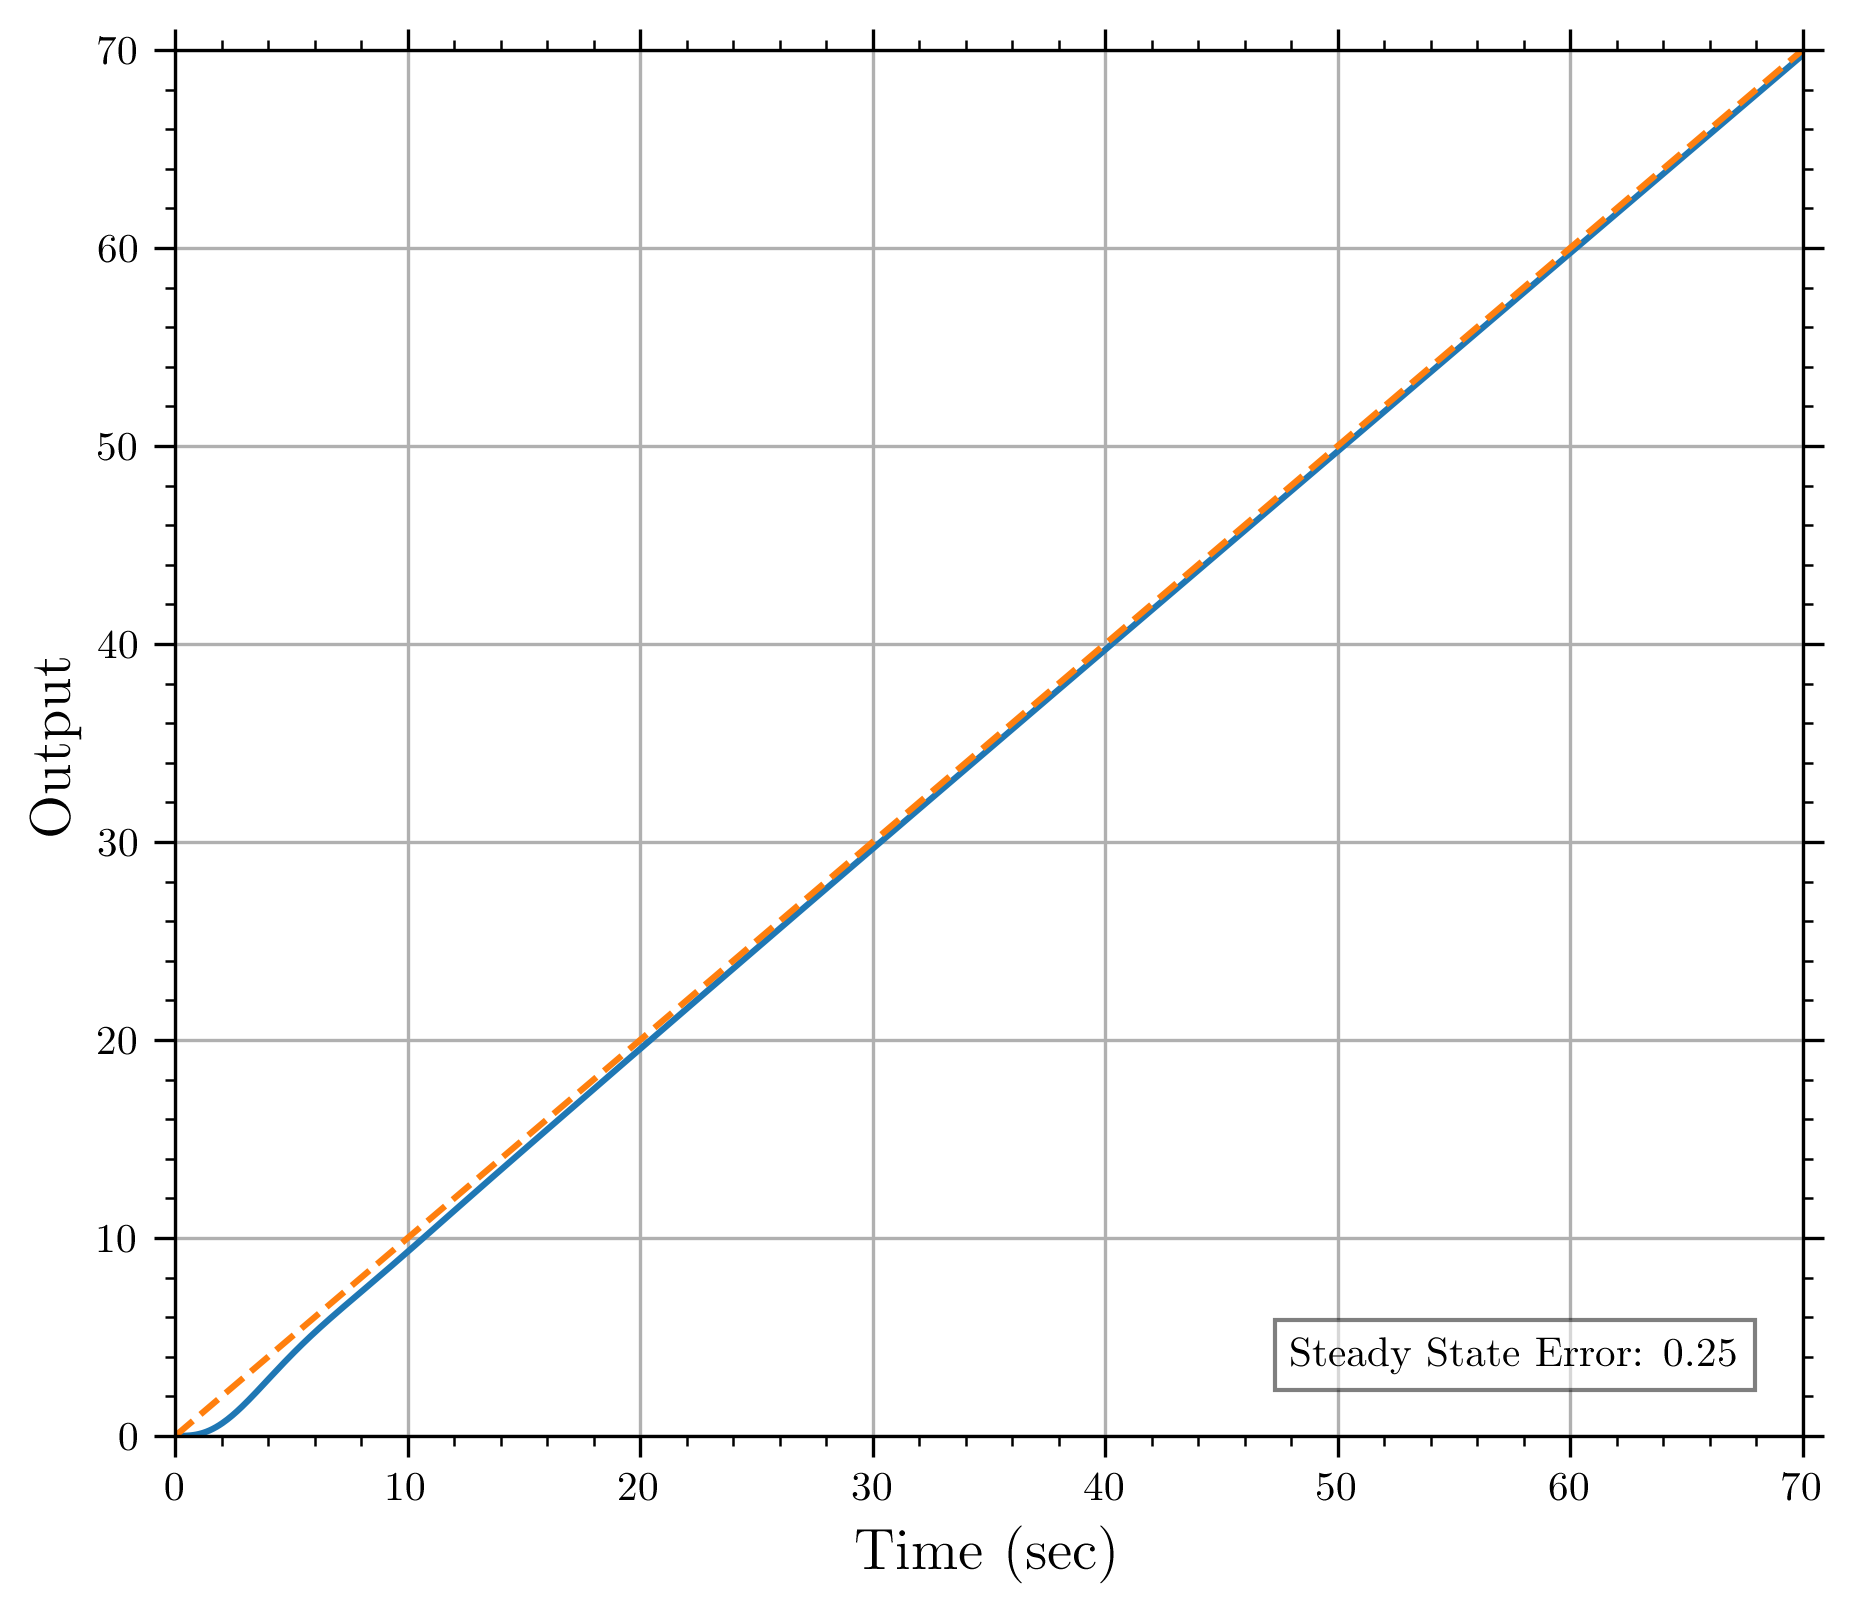
\includegraphics[width=0.7\linewidth]{ramp_response_compensated.png}
    \caption {Ramp response of the compensated system}
    \label{fig:ramp_compensated}
\end{figure}

\section{Conclusion}
We can see that the design requirements have been met, with a gain margin of
$21.24$ dB $\geq 8$ dB and a phase margin of $45.46^\circ > 45^\circ$.

By varying the amount of phase margin, we can achieve different compensators
that can accomplish the same task. Below is a plot of admissible
$\phi_{\text{max}}$ and $\omega_{\text{max}}$ that can be taken to achieve the
desired gain margin and phase margins. Where $\phi_{\text{max}} =
    \sin^{-1}\left(\dfrac{1-a}{1+a}\right)$ and $\omega_{\text{max}} =
    \dfrac{1}{\tau\sqrt{a}}$, for a lag compensator ($a<1$) of the form $G_c(s) =
    \dfrac{a\tau s+1}{\tau s+1}$.

\begin{figure}[h!]
    \centering
    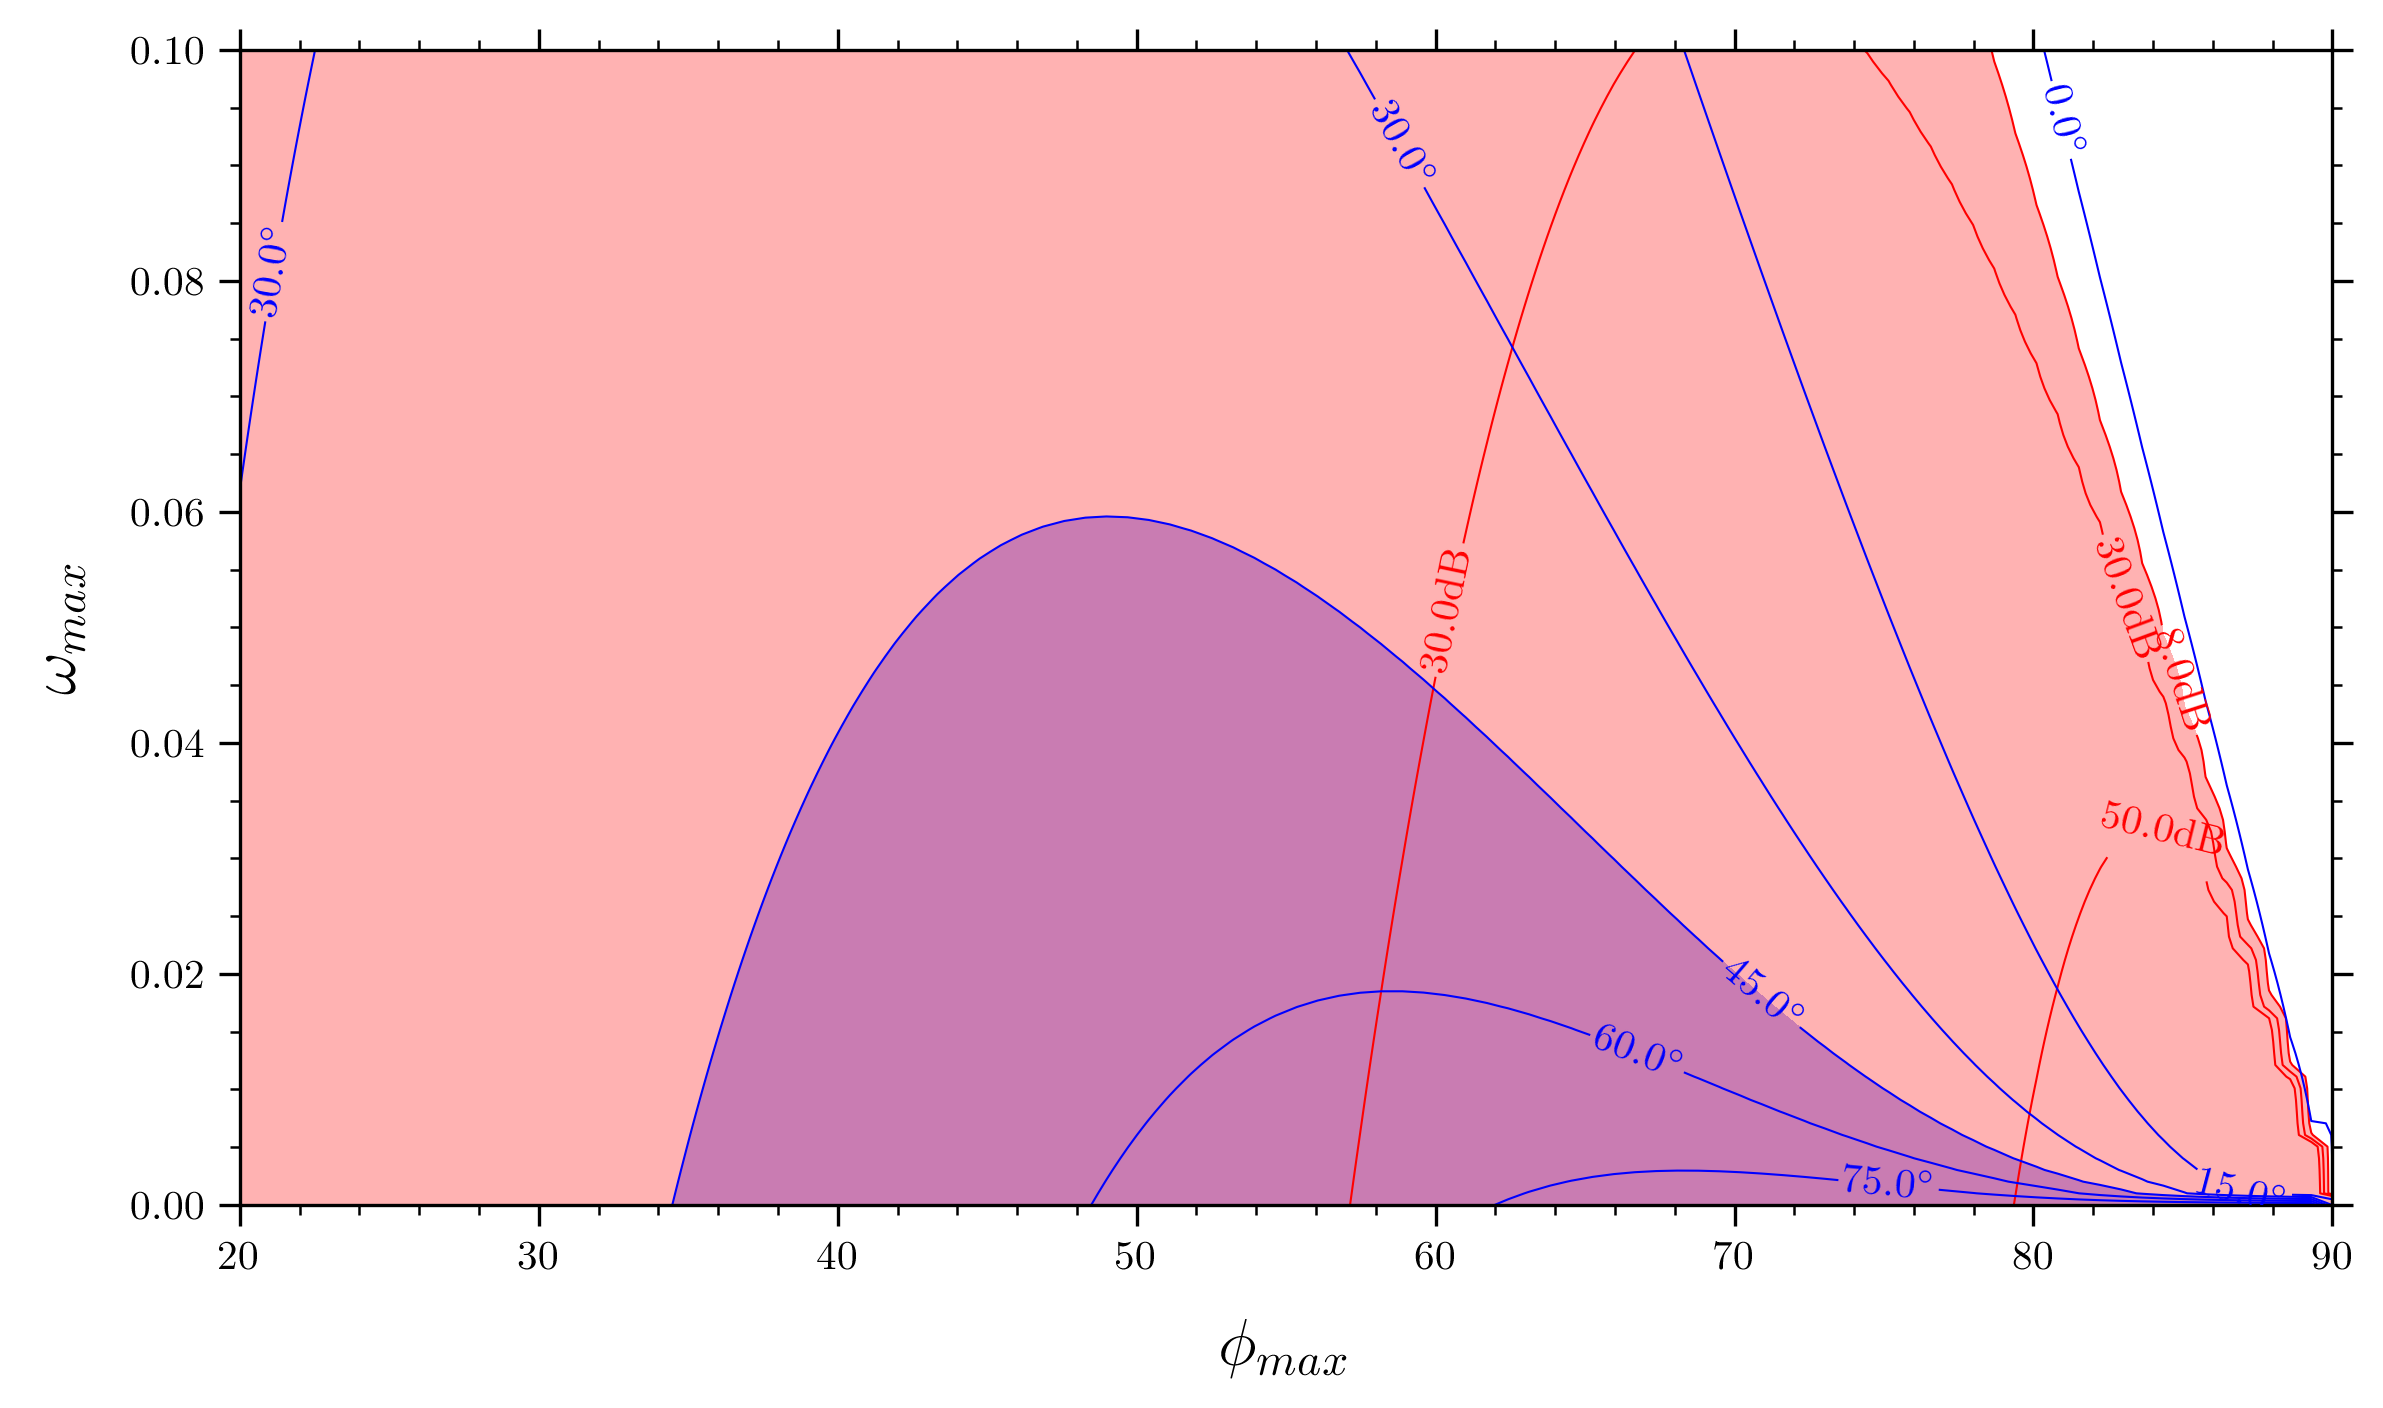
\includegraphics[width=0.8\linewidth]{contour_gm_pm.png}
    \caption {Contours of constant gain margin and phase margins}
    \label{fig:countour}
\end{figure}

Any value of $\phi_{\text{max}}$ and $\omega_{\text{max}}$ that lie in the
common region of the two contours (red and blue) will satisfy the design
requirements.
\end{document}